\documentclass{article}

\usepackage[margin=0.75in, headheight=35pt, includehead, includefoot]{geometry}

\usepackage{fancyhdr}
\usepackage[T1]{fontenc}
\usepackage[shortlabels]{enumitem}
\usepackage{graphicx}
\graphicspath{ {./} }
\usepackage[export]{adjustbox}
\usepackage{booktabs}
\usepackage{forest}
\usepackage{listings}
\lstset{escapeinside={(*@}{@*)}, showstringspaces=false}

\setlength{\parindent}{4em}
\setlength{\parskip}{1em}

\pagestyle{fancy}
\rhead{Alex Kitsul\\230134210\\March 23, 2022}

\begin{document}
\thispagestyle{empty}
\begin{center}
\topskip0pt
\vspace*{\fill}
\Huge Alex Kitsul\\
\Huge 230134210\\
\Huge CPSC 450\\
\Huge Assignment 5 - Report\\
\Huge March 23\\
\vspace*{\fill}
\end{center}
\pagebreak

\section*{Psedocode}
\begin{lstlisting}
main:
    string <- from file

    char_list <- pre_process_string(string)
    fixed_string <- BWT(char_list)
	
pre_process_string(string):
    char_list <- convert string to char list
    letter_count = dictionary of letter occurance counts

    for i from 0 to len(char_list):
        update letter_count for char_list[i]
        char_list[i] = char_list[i] concat letter_count

    if no dollar sign in count, throw error
    return char_list
			
BWT(char_list):
    unsorted_list <- char_list
    sorted_list <- alphabetically sort char_list with $ first
    dict_list <- (keys = sorted_list, values = unsorted_list)
    new_string <- ""

    start <- "$1"
    new_string = new_string concat start[0]

    while dict_list[start] != "$1":
        new_string = new_string concat dict_list[start][0]
        start = dict_list[start]

    return reverse of new_string

\end{lstlisting}

\pagebreak

\section*{Program Code}
\textbf{\underline{BurrowsWheelerTransform}}
\lstinputlisting[language=Python]{../BurrowsWheelerTransform.py}

\pagebreak

\section*{Examples with Output}
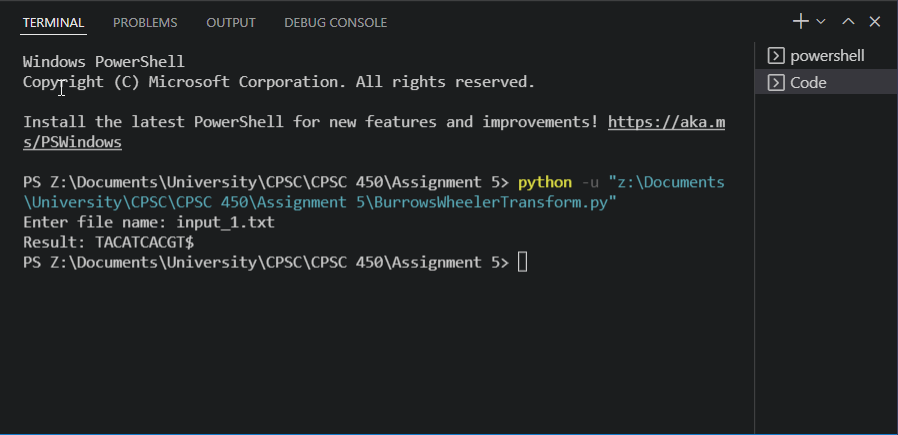
\includegraphics[scale=0.55]{input_1.png}\\
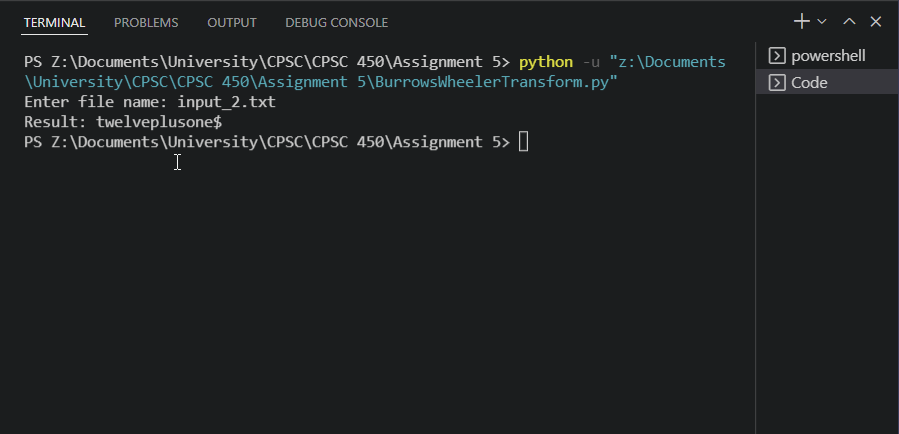
\includegraphics[scale=0.55]{input_2.png}\\
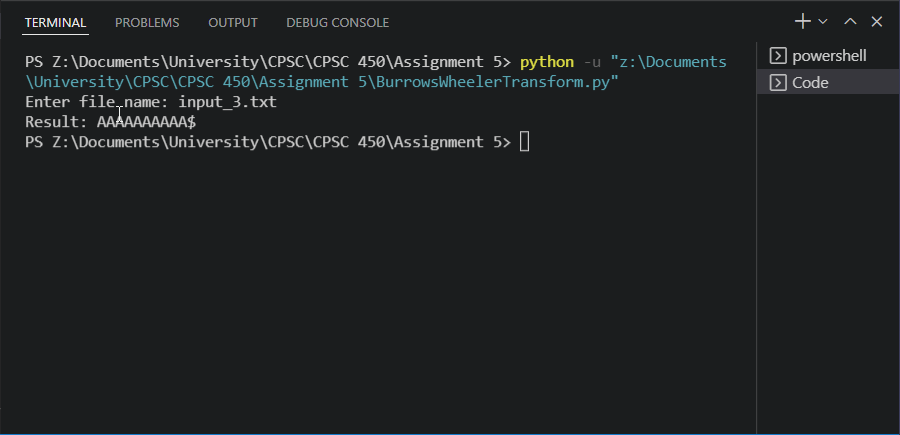
\includegraphics[scale=0.55]{input_3.png}\\

\end{document}
